%%%%%%%%%%%%%%%%%%%%%%%%%%%%%%%%%%%%%%%%%%%%%%%%%%%%%%%%%%%%%%%%%%
%%%%%%%% Final Paper for Penn Machine Learning - Based on ICML 2014 template %%%%%%%%%%%%%%%%%
%%%%%%%%%%%%%%%%%%%%%%%%%%%%%%%%%%%%%%%%%%%%%%%%%%%%%%%%%%%%%%%%%%

% If you rely on Latex2e packages, like most modern people use this:
\documentclass{article}

% use Times
\usepackage{times}
% For figures
\usepackage{graphicx} % more modern
%\usepackage{epsfig} % less modern
\usepackage{subfigure} 

% For citations
\usepackage{natbib}

% For algorithms
\usepackage{algorithm}
\usepackage{algorithmic}

% As of 2011, we use the hyperref package to produce hyperlinks in the
% resulting PDF.  If this breaks your system, please commend out the
% following usepackage line and replace \usepackage{icml2014} with
% \usepackage[nohyperref]{icml2014} above.
\usepackage{hyperref}

% Packages hyperref and algorithmic misbehave sometimes.  We can fix
% this with the following command.
\newcommand{\theHalgorithm}{\arabic{algorithm}}

% Employ the following version of the ``usepackage'' statement for
% submitting the draft version of the paper for review.  This will set
% the note in the first column to ``Under review.  Do not distribute.''
\usepackage{pennML2015} 

% Added to make the table
\usepackage{multirow}

% The \icmltitle you define below is probably too long as a header.
% Therefore, a short form for the running title is supplied here:
\icmltitlerunning{Abraham, Hurwitz, Sankar}

\begin{document} 

\twocolumn[
\icmltitle{Final Project for CIS 419\\Selecting the Optimal Shortest Path Algorithm for Road Networks}

% It is OKAY to include author information, even for blind
% submissions: the style file will automatically remove it for you
% unless you've provided the [accepted] option to the icml2014
% package.
\icmlauthor{Reuben Abraham}{reubenab@seas.upenn.edu}
\icmlauthor{Jordan Hurwitz}{nsankar@seas.upenn.edu}
\icmlauthor{Nivedita Sankar}{jhurwitz@sas.upenn.edu}

% You may provide any keywords that you 
% find helpful for describing your paper; these are used to populate 
% the "keywords" metadata in the PDF but will not be shown in the document
\icmlkeywords{boring formatting information, machine learning}

\vskip 0.3in
]

\begin{abstract} 
We implemented a classifier to determine the fastest single-source, single-target shortest path algorithm for a given road network in the context of optimizing the response times of emergency responder units. We explore the viability of this solution by training several classifiers, including two variations of the Support Vector Machine (SVM) classifier, a standard decision tree, and a boosted decision tree on variations of Djikstra's shortest path algorithm and the A$\star$ algorithm with multiple heuristics.  We evaluated the accuracy, recall, precision, and prediction time to determine the best classifier, and we found that our ultimate choice of XXXXXXX showed promise in most efficiently identifying the fastest shortest path algorithm to use, such that an appropriate path is output. These classifiers draw upon principles from Machine Learning and are relevant for our target application of optimizing emergency responder times. 

\end{abstract} 

\section{Introduction}

Past research efforts in the area of shortest path algorithms in the context of real-world road networks have focused on determining the best general shortest path algorithm. In a study by Zhan and Noon in 1998, a multitude of shortest path algorithms were evaluated on real-world road network data \yrcite{Zhan98}. The paper identified the PAPE graph growth algorithm and variations of Dijkstra as the best general algorithms. However, these results do not take into account the properties of specific graphs. This means today, users must either know about specific features of the graph to decide which algorithm to use, or they must choose an algorithm that works well most of the time.

Often, Dijkstra's shortest path algorithm is used since it is the most general, but alternatives may outperform this choice on select input graphs. However, depending on the feature vectors specific to any given instance of a graph, another algorithm may more efficiently produce the shortest path; for the purposes of this project, we considered variations of Djikstra's, as well as the A$\star$ shortest path algorithm.

We plan to compare the efficiencies of variations of Support Vector Machine and decision tree classifiers, trained on real-world road network data, to determine both the most effective classifier, as well as to triangulate the most efficient shortest path algorithm for an arbitrary road network in working towards the final goal of outputting the optimal shortest path algorithm.

\subsection{Motivation}
Over 1,000 lives are lost every year as a result of delays in emergency response times \yrcite{Blackwell02}. Fast detection of the shortest possible path between a starting point and an emergency destination could contribute significantly towards increasing the speed of emergency responders and thus, their ability to save lives. Given relevant traffic conditions at any particular point in time, the weights of the input road network could be updated to reflect current conditions and provide the emergency response team with the current shortest path.

To achieve this goal, machine learning classifier trained to detect important features of a particular road network given source and target may be able to determine and implement the most efficient shortest path algorithm. In the context of our target application, this may save valuable time that could significantly improve the response times of emergency responders. 

\section{Data Set}

Currently, there is no one universal structure to represent graphs, since often times different applications require different internal graph structures. We chose Graph Modeling Language (GML) because it offers the following advantages: it is easy to read, understand, and parse. Furthermore, there is a lot of graph data available in this format, and many algorithms and packages have already been defined for this structure. We obtained simple GML graphs from Mark Newman's personal website from which to test our parser, and eventually to test our feature extraction. Unfortunately, our input graphs did not have positional data, so in the case of the $A\star$ algorithm, it was difficult to implement heuristics beyond the defaults defined in the \textit{NetworkX} package.

The training and test datasets are extracted from the U.S. Census Bureau's Topologically Integrated Geographic Encoding and Referencing (TIGER) database, and were sourced from the Dryad Digital Repository under the title \textit{Barrington-Leigh-Millard-Ball-PNAS2015-Century-of-sprawl-graphs-in-GML-format}. These data represent real-world street networks, and were output in GML format. Initially, we ran our classifiers on a test dataset of 100 graphs and achieved a maximum accuracy of around 75$\%$, motivating an increase in the size of the dataset. However, we ran into memory errors in trying to parse the 200-graph dataset, leading us to move from batch features to online features.

\section{Feature Generation}

We used Python to preprocess our input data graphs before running them through our supervised learning algorithms. In preprocessing these graphs, we parsed the given graph data in order to obtain feature vectors that represent each graph. We used the \textit{NetworkX} package to obtain most of the following features of our graphs and then combined all of the feature vectors into a 2D \textit{numpy} array, where each column represented values of a particular feature and each row was a different graph. We then passed this numpy array as the X argument in the fit method of our classifier. The features we computed are given below.

\begin{enumerate}
\item Average Clustering
\item Edge-to-Node Ratio
\item Maximum Edge Length
\item Radius
\item Eigenvector Centrality
\end{enumerate}

We further considered Principal Component Analysis for dimensionality reduction, as the bottleneck in running time of this machine learning algorithm is in reading and choosing the features. However, given that we have only extracted a narrow range of features, this approach has limited usefulness.

\section{Algorithms}

\subsection{Shortest Path Algorithms}

For our shortest path algorithms, we chose the standard and bidirectional Djikstra's shortest path algorithms as well as the A$\star$ algorithm. All three algorithms are contained within the NetworkX (NX) package, a Python package designed to handle complex networks. We wanted our three algorithms for comparison to be uniform in their implementation, so we could reliably compare the running times for training and predicting our classifiers. 

\subsection{Learning Algorithms} 

We  chose to sample four different classifiers to compare their performance, given that our target application was to find the shortest geographical path between two points for emergency responders. We believe that these classifiers may be particularly relevant for our purposes because they require only a relatively general base learning algorithm. Therefore, we know that future test data will conform to the road data we used for testing. It is important to remember that certain classifiers, such as Naive Bayes, would be unsuitable since many of the features we have computed over the graphs may be correlated with each other. Once we determined that X was the most appropriate classifier, we tuned its parameters using GridSearch over the training set based on the true labels of the training set. Having chosen this classifier, we compared the prediction results of our classifier on our training set with the true labels for the training data. This comparison enabled us to obtain evaluation metrics including accuracy, precision, and recall, against which to score our classifier and determine its viability as a solution for emergency responders.

\subsection{SVM: Sigmoid and RBF Kernels}

We used two types of support vector machines (SVMs) with radial basis function (RBF). We chose to use support vector machines because we predict that there will be correlation between the graphs, and SVMs are capable of handling data that is not linearly separable. In the case that the final model may not be linear, an SVM with an RBF kernel is generally considered to be a default option. The other common choice of kernel, a sigmoid kernel, which can be used interchangeably with perceptron neural networks, has further been highly effective in practice but may be less applicable for our chosen application. We predicted that the support vector machine classifiers would give us the highest accuracy of all of our classifiers.

\subsection{Decision Tree}

We chose to test a depth-3 decision tree classifier because it can handle the graph features we use as inputs to the base learning algorithm and can split on the shortest path algorithms relatively quickly. Further, a decision tree classifier has the unique benefit of being easy-to-use and user-friendly. An emergency responder would only need to input his starting point in order to use this classifier. However, we recognize that a downside of this approach is the necessity of knowing the features of a graph in order to run this classifier. As a result of this analysis, we predicted that the decision tree classifier would be the fastest of all of our classifiers. We further tested a boosted version of the decision tree to improve accuracy and precision.

\section{Discussion}

We sampled four total variations of SVM and decision tree classifiers, and metrics for their learning accuracy precision, and recall can be found in the next section. For each classifier, we implemented GridSearch to determine the optimal parameters, which are again specified below. However, while GridSearch worked to optimize the test accuracy of each classifier, it resulted in a sacrifice in recall score in some cases, meaning that our classifier always predicted a single algorithm. As a result, in the case of the boosted decision tree and the SVM with a radial basis function kernel, we manually adjusted the parameters to find a classifier with the greatest consolidated accuracy, precision, and recall scores.

\subsection{Error Rates}

ROC curves demonstrate the ability of a classifier to effectively separate input data graphs by their respective most efficient algorithm. The higher the area under the ROC curve, the more effective the test result. Figure 1 below demonstrates the Receiver Operating Characteristic (ROC) curve given the GridSearch-chosen parameters for our SVM, decision tree, and boosted decision tree classifiers. As evident below, the SVM with an RBF kernel has the highest accuracy for GridSearch-chosen parameters.

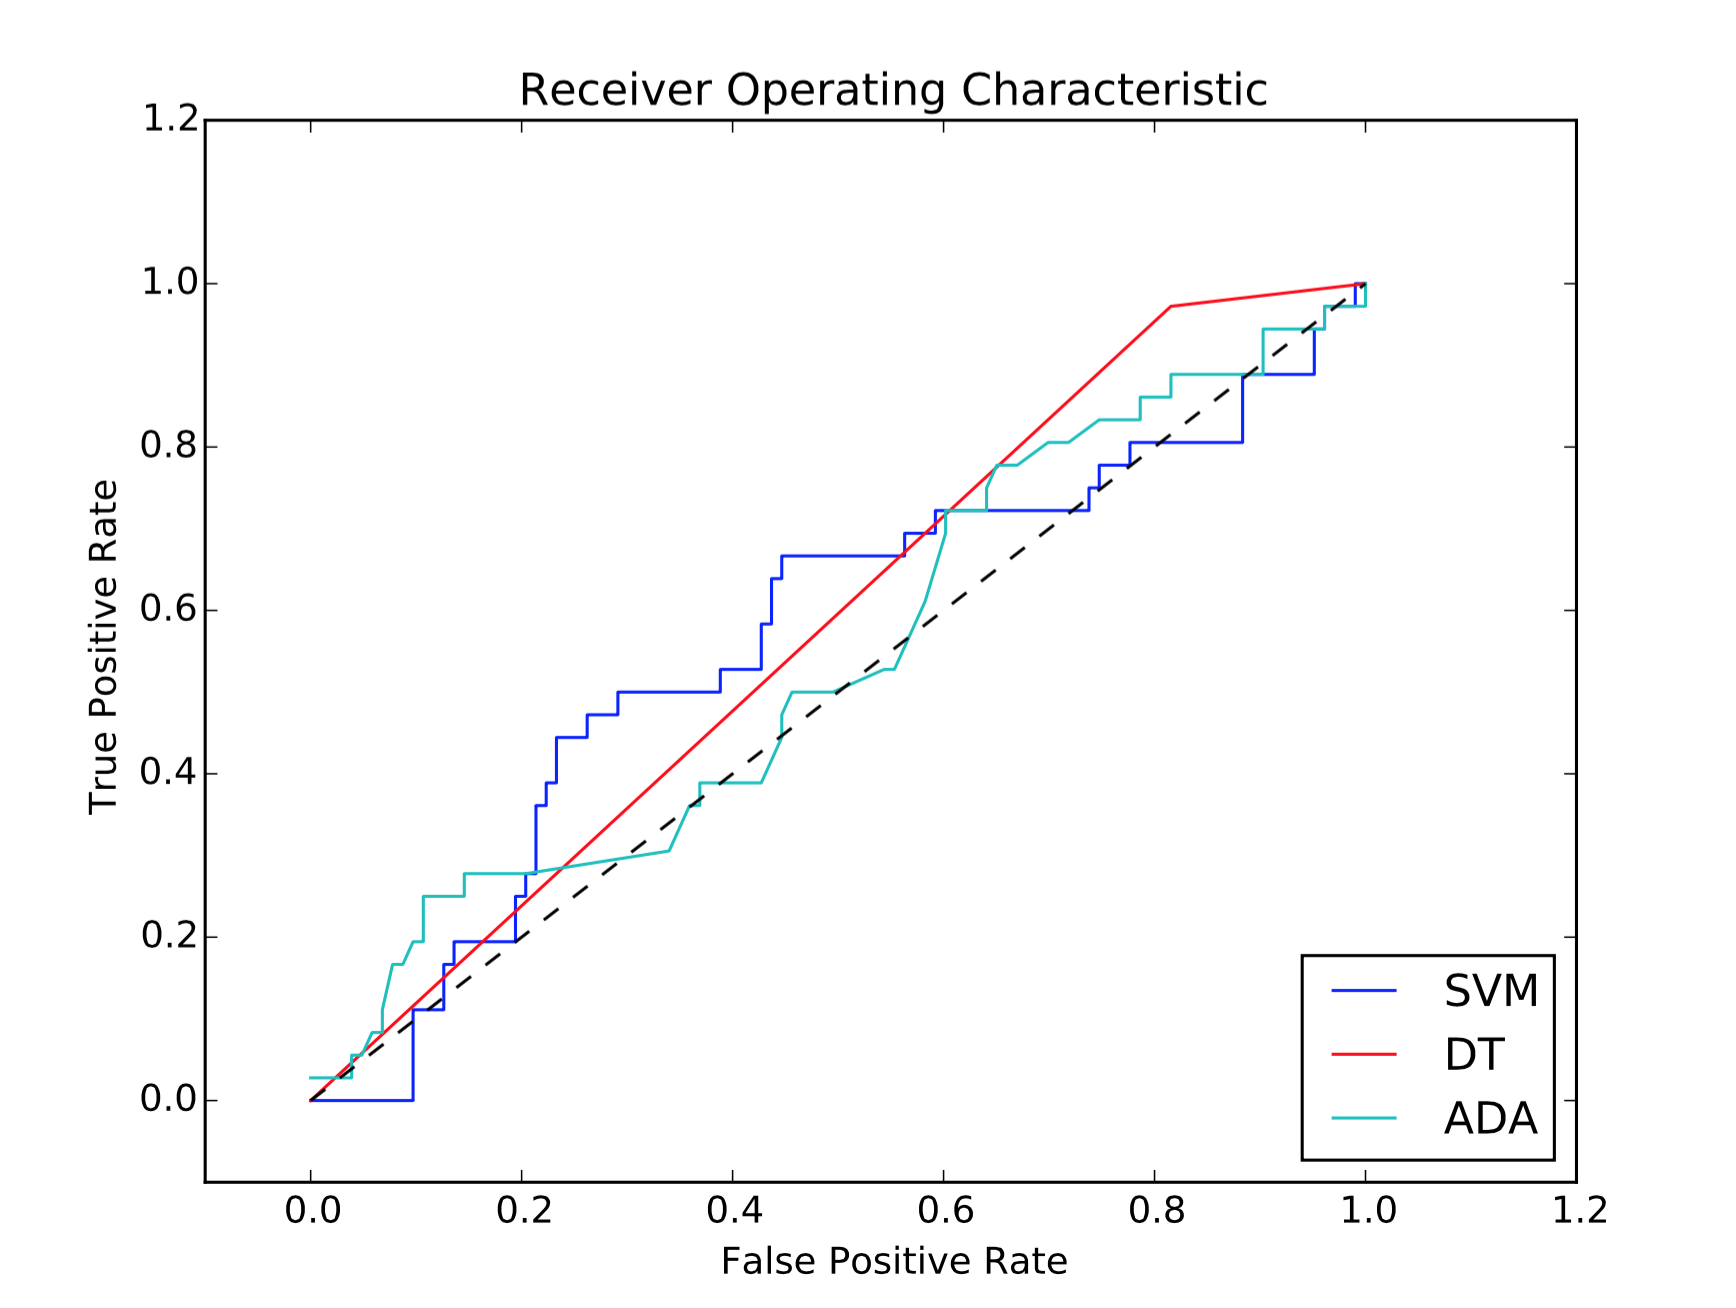
\includegraphics[width=8.5cm]{ROC}

Figure 2 below represents the ROC curve given the manually optimized parameters for our SVM, decision tree, and boosted decision tree classifiers. Once these parameters were manually adjusted to improve test recall for the AdaBoost and SVM classifiers, it is clear that the depth-3 decision tree has the highest accuracy. However, the AdaBoost and SVM classifiers with manually adjusted parameters are viewed as more effective classifiers than their GridSearch-optimized counterparts because they are more discriminating in instances, as reflected in the their lower recall scores.

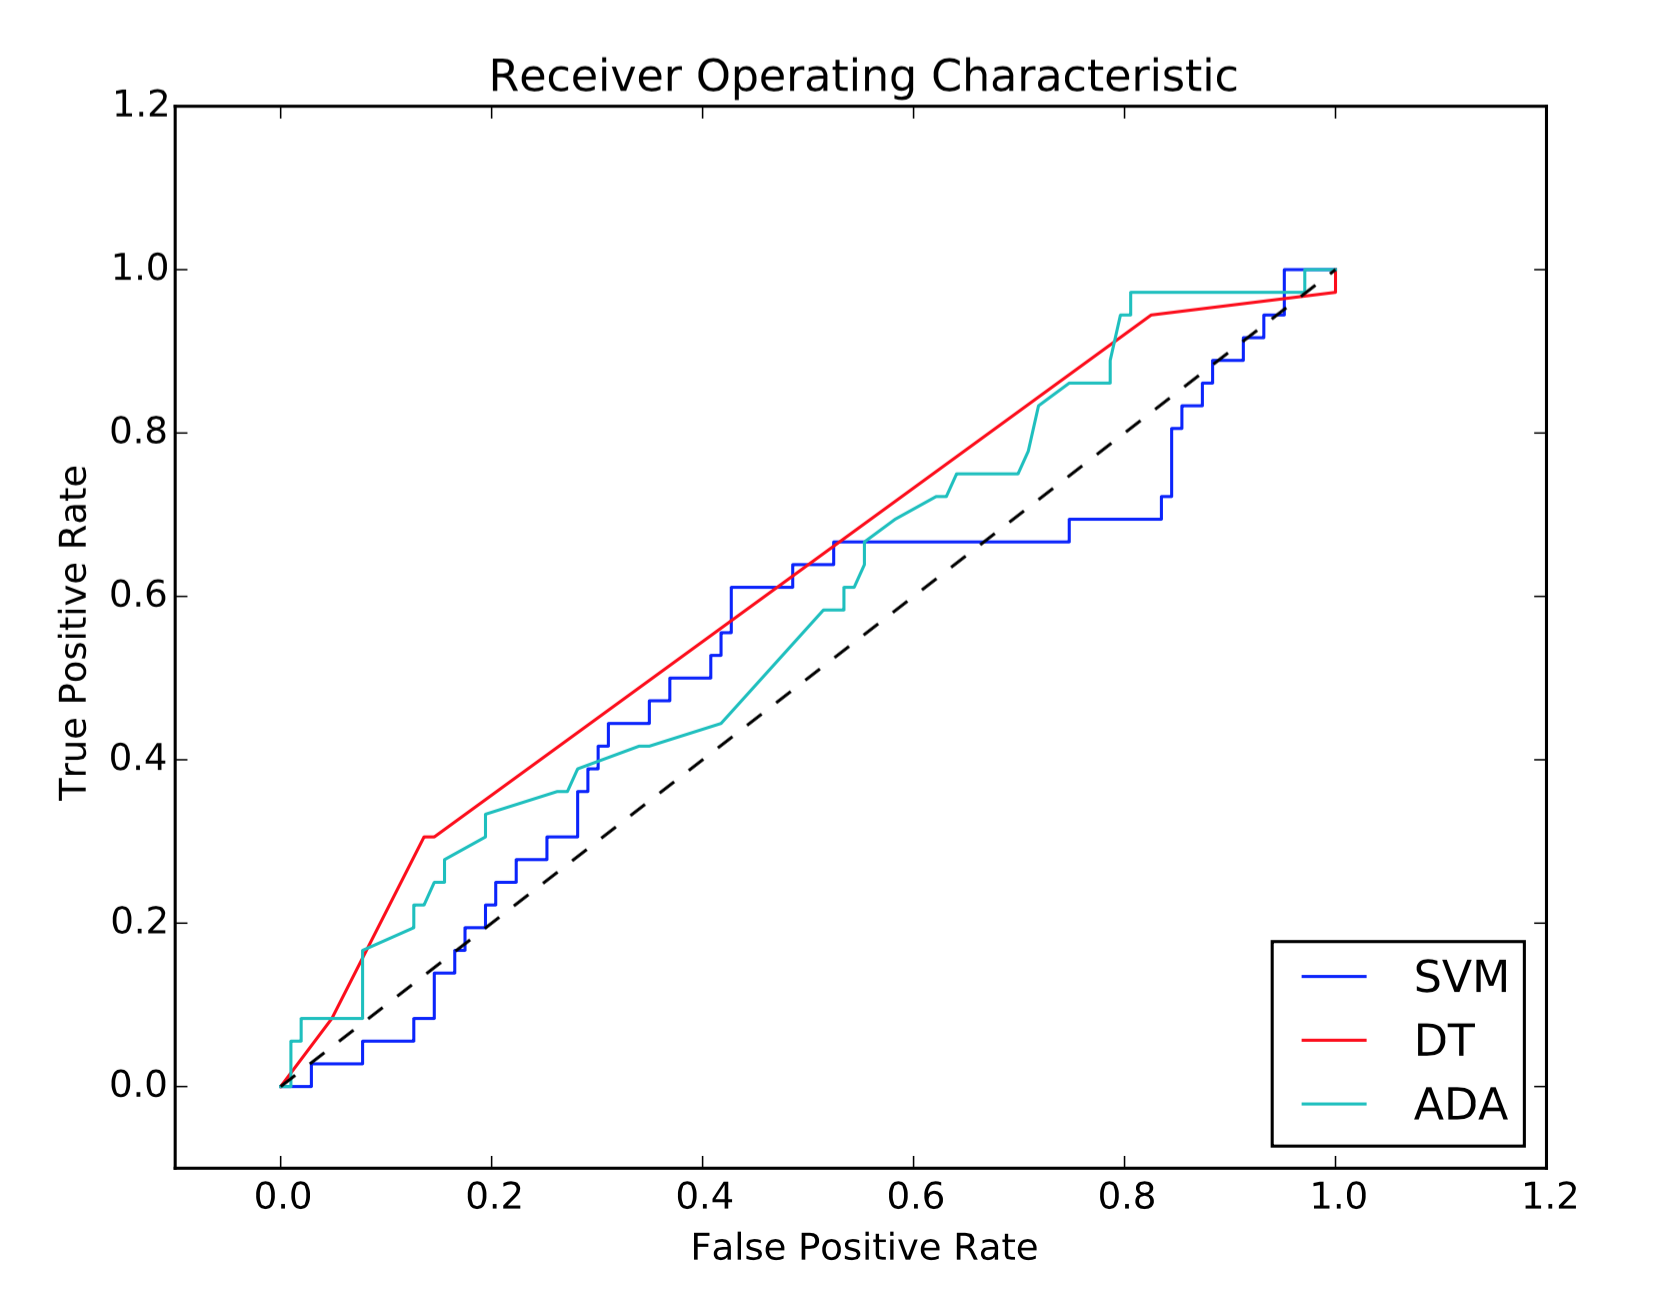
\includegraphics[width=8.5cm]{ROC2}

The full accuracy, precision, and recall metrics for each of our classifiers are given in Tables 1-3 below.

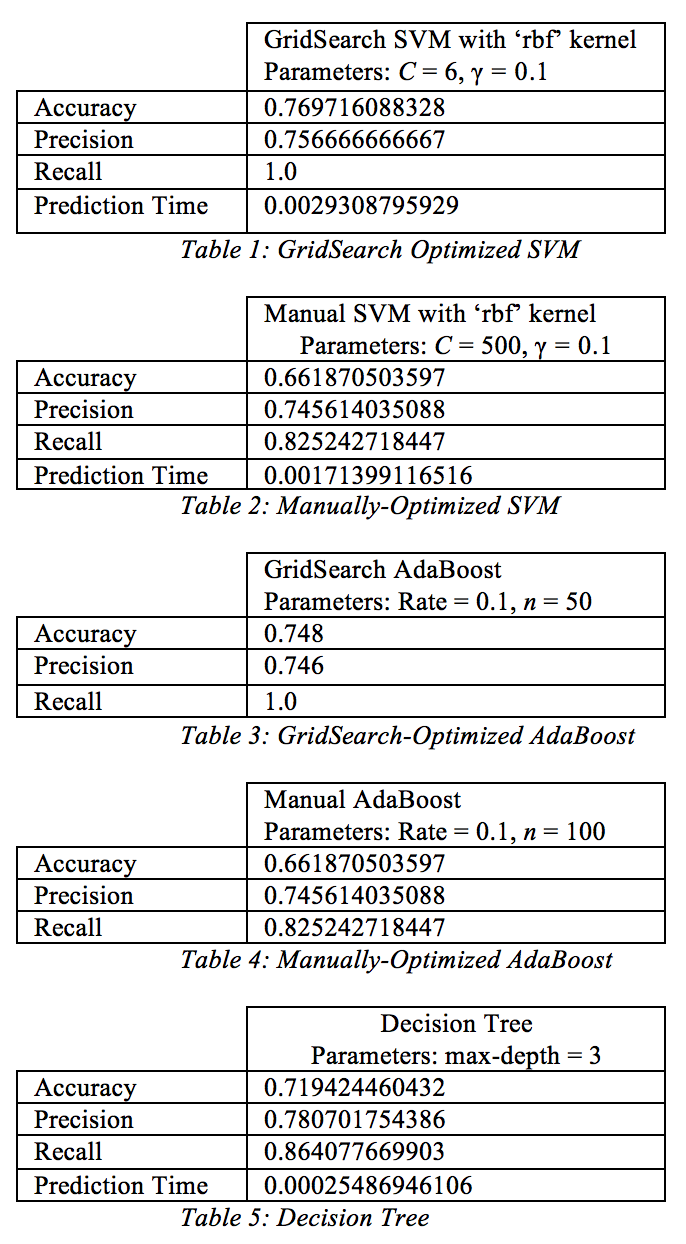
\includegraphics[width=8.5cm]{tables}

\subsection{Experimental Results}

Having optimized the accuracy, precision, and recall ratios of our classifiers, we found that a depth-3 decision tree had a lower prediction time than did the SVM classifier and, by definition, the AdaBoost classifier, meaning that it separated test instances more quickly than our other chosen classifiers. This classifier had a 72\% accuracy and predicted a shortest path algorithm in 0.00025 seconds, 

\section{Algorithm Preference}

Given that the depth-3 decision tree had the strongest performance of our sampled classifiers, we ran 

\section{Evaluation and Analysis}

\section{Conclusions}



\bibliography{final_paper}
\bibliographystyle{icml2014}

\end{document} 


% This document was modified from the file originally made available by
% Pat Langley and Andrea Danyluk for ICML-2K. This version was
% created by Lise Getoor and Tobias Scheffer, it was slightly modified  
% from the 2010 version by Thorsten Joachims & Johannes Fuernkranz, 
% slightly modified from the 2009 version by Kiri Wagstaff and 
% Sam Roweis's 2008 version, which is slightly modified from 
% Prasad Tadepalli's 2007 version which is a lightly 
% changed version of the previous year's version by Andrew Moore, 
% which was in turn edited from those of Kristian Kersting and 
% Codrina Lauth. Alex Smola contributed to the algorithmic style files